\documentclass[11pt]{article} % do not change this line
\input{BigDataStyle.txt}      % do not change this line
\usepackage{amsmath,amsfonts,amssymb,amsthm,latexsym,graphicx,caption,hyperref,listings,color}
\usepackage[boxed,ruled,vlined,dotocloa,english,onelanguage]{algorithm2e}
\graphicspath{ {pictures/} }
\emergencystretch=5mm
\tolerance=400
\allowdisplaybreaks[4]

\theoremstyle{plain}
\newtheorem{theorem}{Theorem}[section]
\newtheorem{proposition}[theorem]{Proposition}
\newtheorem{corollary}[theorem]{Corollary}
\newtheorem{lemma}[theorem]{Lemma}
\newtheorem{problem}[theorem]{Problem}
\newtheorem{definition}{Definition}[section]

\theoremstyle{definition}
\newtheorem*{remark}{Remark}

\title{Analysis of Symmetry Breaking Algorithms in Distributed Synchronous Systems}
\author{Marcos Tileria}

\newcommand{\Programme}{MSc Distributed and Networked Systems}
% Computational Finance students: uncomment the next line
%\twodepartmentstrue

\begin{document}
\maketitle

\declaration

\begin{abstract}
  
 Symmetry Breaking is a well studied problem in distributed computing. A distributed system presents a symmetry when all processes share the same state. The goal of symmetry breaking algorithm  is to break the state of equilibrium of a distributed system before the start of a computation. The objective of this dissertation is to analyse time and message complexity of distributed symmetry breaking algorithms on synchronous systems, in particular the Maximal Independent Set problem, which results to be one of the most important symmetry breaking problems. Three types of synchronization techniques are used to simulate a synchronous system over an asynchronous message passing system. A simulator developed in the Elixir was built in order to analyse the problem using different synchronization techniques. The results of the simulation show that ..... and present the trade off among the synchronization techniques.... TBC
  

\end{abstract}



\section{Introduction}
\label{cap:1}

One of the central problem in distributed computing is called Symmetry Breaking. This problem occurs when all processors in a network are in the same state, possibly with a unique identifier. This state of symmetry should be broken before beginning any computation. Some examples of symmetry breaking problems are computing the maximal independent sets \textit{(MIS)} , maximal matching, vertex colouring, ruling sets and leader election. This project focus on the problem of finding the maximal independent set on an undirected graph using the local model \cite{linial1992locality}.

In the local model, each vertex of the graph is occupied by a processor and has a unique identifier ID. The processors only communicate with each other by sending messages, there is no notion of shared memory. Locality in distributed networks means that in order to obtain the solution of a general problem, a processor only uses locally available data. In this model, computation is assumed to be reliable and synchronous. No faulty processors are permitted in this model and every processor executes the local algorithm in steps call rounds. 

An independent set \textit{IS} of an undirected graph is a subset S of nodes such that no two nodes in S are adjacent. An \textit{IS} is considered maximal if no extra node can be added to \textit{IS} without violating the independence. The \textit{MIS} problem is one of the most important problem in the area of local graph algorithm because many other problems like graph colouring can be reduced to it \cite{panconesi1992improved}. A maximum independent set \textit{MaxIS} is a \textit{MIS} of maximum cardinality, this problem, in contrast to \textit{MIS} in NP-hard. In this project a random-priority parallel algorithm developed by Yves \textit{et al.} \cite{yves2009optimal} is used in order to find the MIS of a given graph.


There are many applications of the \textit{MIS}, for instance: resource scheduling, topology control in wireless sensor networks \cite{basagni2001finding}, analysis of biological systems \cite{afek2013beeping}. Karp and Wigderson \cite{karp1986constructing} presented reductions from others graph theory problems (Maximal Set Packing, Maximal Matching, 2-Satisfiability) to the \textit{MIS} and proved that the \textit{MIS} problem is in NC.


In practice, the majority of the distributed systems are asynchronous, however, protocols are easy to design and implement in the synchronous model. Once that an algorithm has been designed in the synchronous model it can be transformed to an asynchronous algorithm.  The main reason why synchronous algorithms are easy to design is that the model makes strong assumptions and put constraints that restrict the behaviour of the system.


There are many techniques to simulate a synchronous system over an asynchronous system. A synchronizer is a simulation from the synchronous system to the asynchronous system. These simulations can be local or global. In a local simulation, processors only keep the synchronization with its neighbours, on the contrary, on global simulations all processors are synchronized.  For this reason, with local synchronization, especially in large networks, processors might be in different rounds. For this project, two well know synchronizers proposed by Awerbuch \cite{awerbuch1985complexity} are used, Alpha and Beta Synchronizer. Besides, a global synchronizer with a master processor that controls the synchronization was implemented to analyse the overhead generated by different techniques in terms of messages and time.




The rest of the report is organised as follow: The next section presents relevant work about symmetry breaking, maximal independent set and synchronizers. Section \ref{cap:2} presents the background of symmetry breaking and define the MIS problem. Different approaches to simulate synchronous systems are discussed in Section \ref{chap:3}. A description of the simulator and a tutorial on how to use it is given in section \ref{chap:4} The experimental settings of the simulations are explained in Section \ref{chap:5}. Section \ref{chap:6} gives the evaluation of results and conclusion. Finally, the professional issues are presented in Section \ref{chap:7}. 

\subsection{Background Research}
 
Deterministic and randomised algorithms are two well studied approaches to solve symmetry breaking problem. Usually, randomisation provide simpler and faster implementation than the deterministic counterpart. Deterministic algorithm always reaches the solution of the problem, in contrast, randomised algorithms achieve termination with high probability. Relevant work, especially the ones related to \textit{MIS} problem are quoted below.

In \cite{luby1986simple}, Luby proposes the first solution to the \textit{MIS} problem using a simple randomised algorithm. The same year Alon \textit{et al.} present in \cite{alon1986fast} another randomised solution and made a comparison with others algorithms that were turned from randomised to deterministic. Both algorithms run in $O(\log |N|)$ in general graphs. In \cite{linial1992locality} Linial present a $\Omega(\log* |N|)$ algorithm to find the MIS for n-cycle graphs. A deterministic solutions was presented by Panaconesi \textit{et al.} in \cite{panconesi1996complexity} that run in $2^{O\sqrt{\log N}}$, more recently, many deterministic algorithms were presented by Barenboim and Elkin in \cite{barenboim2010sublogarithmic} with different running times for different network topologies. Schneider and Wattenhofer developed a $O(\log^* N)$ deterministic algorithm for graphs with bounded growth in \cite{barenboim2010sublogarithmic}. In \cite{yves2009optimal}, Ives \textit{et al.} present a variant of the original Luby's algorithm with optimal bit complexity for the messages sent over the network, this algorithm is used in this project for testing purpose.

 

In \cite{awerbuch1985complexity}, Awerbuch present a general simulation technique to allow the implementation of algorithm in synchronous networks, referred to as synchronizer. In this paper, the author present three synchronizer Alpha, Beta and Gama, which are a generalisation of the work of Gallager and Robert in \cite{gallager1982distributed}. Logical buffering is another technique to simulate synchronization and was independently developed by Welch in \cite{welch1987simulating} and Neier and Toueg in \cite{neiger1993simulating}. Others techniques were developed improving the synchronizer mention before under some restrictions, for example, Peleg in \cite{peleg1989optimal} for multidimensional mesh network with two nodes in each dimension(hyper-cube).

 Barenboim \textit{et al.} made in \cite{barenboim2016locality} a survey of symmetry breaking algorithms describing the main results achieved on the topic and proposed new algorithms for the most popular symmetry breaking problems: \textit{MIS}, maximal matching, vertex colouring and ruling sets. In \cite{johnson1985symmetry} Johnson and Schneider present a discussion to address the meaning of symmetry and introduce the concept of similarity.  
\newline
% \newpage



\section{The Symmetry Breaking Problem}
\label{cap:2}

Formally, a symmetry system can be defined as a system in which the processes are in an equivalence relation, this means that if the processes run the same code, it is possible to permute the processes without changing the behaviour of the system. One example of this state would be a ring in which there is no unique identifier for every processes \cite{boldi1996symmetry}. 

If we consider a message passing system in which exist an initial state of symmetry between all processes, it is possible to find a synchronous execution in which the processes will continue in the same initial state. In this case, it is necessary a mechanism to break the symmetry, on the contrary, the system cannot escape from the initial state.
%as shown in \cite{angluin1980local} by Angluin.

Symmetry breaking is one of the most extensively studied problems in distributed computing. The fundamental problems on graph include the maximal matching, vertex colouring, ruling sets and \textit{MIS}. The last one can be considered as the central problem because all the others can be reduced to it, as shown in  \cite{linial1992locality}.

In the next section, a formal definition of the maximal independent set is given. A  discussion on the sequential algorithm vs distributed algorithm is presented with the theoretical analysis on time complexity and message complexity in the case of the distributed approach. Henceforth the terms vertices and processes are used in the same context and are interchangeable.    

\subsection{Maximal Independent Set}

\theoremstyle{definition}
\begin{definition}

Given a undirected graph $G = (V,E)$, a Maximal Independent Set \textbf{MIS} is a set of vertices $S \subseteq V$ if it satisfied the following properties:   

\begin{enumerate}
  \item the set S in an independent set meaning that no two vertices $v,u \in S$ are adjacent,
  \item the set S is maximal, with regards to independence, meaning that for each vertex $v \notin S$, there exist a neighbour $u$ of $v$ such that $u \in S$.
\end{enumerate}

\end{definition}

REWRITE THIS PARAGRAPH
Figure \ref{fig:graph1} show an example of undirected graph $G$ with 8 vertices and 14 edges. The goal is to find a MIS of $G$, informally, a set of vertices in which every vertex $v$ is part of the set or a neighbour of $v$ is part of the set. It is possible to find more that one solution to the same instance as shown in the example.
 
\begin{figure}[ht]
\centering
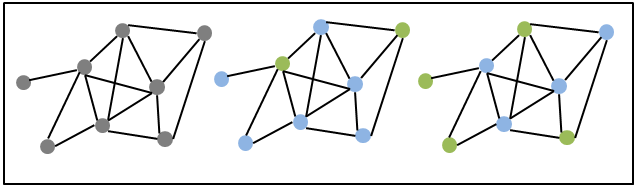
\includegraphics[width=1 \linewidth, height=5cm]{mis-example.PNG} 
\caption{Maximal Independent Set of a general graph}
\label{fig:graph1}
\end{figure}


The algorithm \ref{algorithm:secuential-mis} describe a general sequential algorithm to find the maximal independent set of a general graph. The time complexity is $O(N)$ since in the worst case, the algorithm has to check every vertex. Another approach to improve this time is desirable. In the next section, two distributed algorithm to find the \textit{MIS} are presented.

\begin{algorithm}
 \caption{Sequential Maximal Independent Set}
 \label{algorithm:secuential-mis} 

\SetAlgoNoLine
\KwResult{IS Set of vertices}
\KwData{ $G(V,E)$ Graph}
    \While {V is not empty}{
        Choose a vertex $v \in V$
            Add v to the set IS\;
            Remove from V the vertex v and all its neighbours\;
        }
    
 
\end{algorithm}
 
 


 
\subsection{Distributed Maximal Independent Set}

A logarithmic lower bound is always desirable to solve a problem optimally, for this reason, the difficulty to find it in sequential algorithms motivated the proposal of distributed algorithms. In distributed computing, randomised algorithm is a powerful and efficient technique to solve efficiently problem that may take longer time in deterministic approach.

In 1986, a efficient distributed algorithm was proposed independently by Luby \cite{luby1986simple} and Alon \textit{et al.} \cite{alon1986fast}. Both algorithms are randomised and have $O(log N)$ lower bound. Until now, there are faster than the best deterministic algorithms for general graphs. There have been some improvements for special cases, for instance, \cite{panconesi1996complexity} propose a $O(\delta + log^* N)$ algorithm for specific graphs, however, the original algorithms are still faster when the running time is expressed as a function of $N$. It is worth to mention that all algorithms exposed forward are in the synchronous model.  

The algorithm\ref{algorithm:luby-mis} describe the original Luby's algorithm. Show the correctness of this algorithm is very simple. In each round, if a vertex joins the set \textit{S}, no other neighbour join the set in the actual round or in any other round. The algorithm at the end produces a \textit{MIS} because the vertices with the highest degree will decide to enter the \textit{MIS} in each round until all vertices become inactive.

% If Luby’s algorithm ever
% terminates, then the final set S satisfies the
% independence property.

% Theorem 6: If Luby’s algorithm ever
% terminates, then the final set S satisfies the
% maximality property.

% \theoremstyle{definition}
\begin{definition}

An algorithm terminates w.h.p. (with high probability) within $O(t)$ time if it does so with probability at least $1 − 1/n^c$ for any choice of $c ≥ 1$.

\end{definition}

 Message complexity depends on the number of processes which are active in each phase and its denoted by $O(m)$ in \cite{luby1986simple}. With high probability $(1-1/n)$, the Luby's algorithm finishes  $4\log N$ round. The time complexity demonstration is omitted FOR THE MOMENT.

% \theoremstyle{theorem}
\begin{theorem}

Algorithm \ref{algorithm:luby-mis} computes a maximal independent set for any graph  in $O(\log n)$  rounds with high probability.

\end{theorem}


\begin{algorithm}
 \caption{Luby's Algorithm, code for each process $p_i$ i = 1 to N}
 \label{algorithm:luby-mis} 

\SetAlgoNoLine
\KwResult{MIS Maximal Independent Set}
\KwData{ $G(V,E)$ Graph}
    \While {V is not empty}{
        Choose a random set of vertices $S ⊆ V$, by selecting each vertex $v$ independently with probability $1/(2d(v))$, where d is the degree of $v$\;
        For every edge in E, if both its endpoints are in the random set S, then remove from S the endpoint whose degree is lower. Break ties arbitrarily, e.g. using a lexicographic order on the vertex names\;
        Add the set S to IS\;
        Remove from V the set S and all the neighbours of vertices in S\;
        }
\end{algorithm} 



The algorithm \ref{algorithm:main-mis} is another randomized distributed algorithm and was proposed by Yves \cite{yves2009optimal}. This algorithm is used for the simulations in this project. The rounds can be split into 2 phases for simplicity. In each phase, each process chooses a random value, send to its neighbours and wait to receive the value from all its neighbours. If the process has the maximum value, the join the set and output in. In the second phase, if the process decided to join the $MIS$, then send messages to all its actives neighbours. If the process receives a message from one neighbour, decide not join the MIS and output out. At the end of this phase, every process that made a decision about join or not the \textit{MIS} become inactive for the next rounds.

\begin{algorithm}
 \caption{MIS Algorithm, code for each process $p_i$ from i = 1 to N}
 \label{algorithm:main-mis} 

\SetAlgoNoLine
\KwResult{MIS Maximal Independent Set}
\KwData{ $G(V,E)$ Graph}
    \While {V is not empty}{
        Selects a random number $r(v)$ between [0,1] and sends to its neighbours\;
        If $r(v) < r(w)$ for all neighbours $w \in N(v)$ numbers, remove myself from V and enter to the MIS \newline
        Inform my neighbours that I am a MIS member and terminate\;
        If I heard that my neighbour is MIS, remove myself from the V and terminate\;
        }
\end{algorithm}

% Lemma 7.14 (Edge Removal). In a single phase, we remove at least half of
% the edges in expectation.

The correctness is very intuitive and similar to the Luby's algorithm. In one phase, one process $p_i$ join the set $S$ only if it has the larger value between its neighbours, at the end of that phase, all the $p_i$ neighbours become inactive. In consequence, there is no neighbour process in the $S$. This set $S$ is maximal because at least one vertex (with the global smallest value) will enter the $S$ per round, hence there is a progress in each round. If at some round, a vertex has no neighbours, automatically join $S$ and become inactive. This sequence continues in following rounds until every process becomes inactive

% \theoremstyle{theorem}
\begin{theorem}

Algorithm \ref{algorithm:main-mis} computes a maximal independent set for any graph in $O(\log n)$ rounds with high probability.

\end{theorem}


% . This algorithm operates in synchronous rounds. In line 2, every process select a random number to in order to break the symmetry with its neighbours, line 3 makes sure that if a vertex v join the MIS, no other neighbour of v join the MIS at the same time, this is true because the execution  occurs in rounds. the line 4 makes sure that any vertex that has a neighbour in the MIS, join the MIS at any point. 


\newpage
% \newpage

\section{Synchronous Distributed Systems}
\label{chap:3}

A synchronous distributed system is ..... TBC

A synchronizer is a general technique to simulate synchronous communication by asynchronous systems. Synchronizer was introduced by Awerbuch \cite{awerbuch1985complexity}, in this paper, the author presented 3 different synchronizers and analysed the trade off between them. This technique allows the execution of distributed synchronous algorithm over an asynchronous system, for instance, an asynchronous message passing system. The reason why synchronous algorithms are desirable is that there are usually simpler to design and superior in complexity. 

The graphic \ref{fig:simulation} shows the interactions between the layers of the simulation. The bottom layer is the asynchronous message passing system, here there is no guarantee on messages delay. A Synchronizer work over this layer. The goal of a synchronizer is to provide the illusion of synchronous system to the upper layer. For this example, the Maximal Independent Set algorithm is the user of the synchronizer. Any layer over the synchronizer can use the primitives \textit{Sync-}$send_i$ and \textit{Sync-}$recv_i$ and safely assume that the communication is synchronous.      

\begin{figure}[ht]
\centering
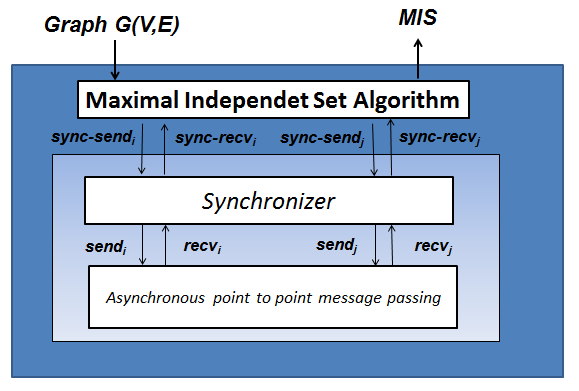
\includegraphics[width=1 \linewidth, height=8cm]{simulation.PNG} 
\caption{Diagram of the simulation of a synchronous distributed systems using synchronizers}
\label{fig:simulation}
\end{figure}


The following model was used in the original paper by Awerbuch \cite{awerbuch1985complexity} and was previously used in \cite{segall1983distributed,gallager1982distributed} among others. The asynchronous system is represented by an undirected graph $G = (V,E)$ where $V$ represent the set of processors and $E$ represent a bi-directional communication channel. Each processor sends messages, receive messages and perform some local computation. There is no notion of how long takes messages to arrive the destination but it is assumed to be finite. Another important assumption of the model is that the amount of information carried by messages is limited.

In this model, processes send messages after they receive a pulse or clock. This pulse represents one time unit (round) in the synchronous system. The delay of the messages in one round is one unit of time of the global clock.

\begin{definition}
\label{def:safe}
A process $p_i$ is said to be safe in a round only after all its messages has been delivered at their destinations.
\end{definition}

If all neighbours of $p_i$ are safe in the round $r$, this mean that $p_i$ has received all messages for $r$. In this case, $p_i$ in ready to execute the $r + 1$ round of the algorithm. This property ensures that from the point of view of the algorithm (that use the synchronizer), the network behaves as a synchronous communication system when really its an asynchronous system, this is why it is call a simulation. An easy solution to detect if a process is safe it is to force each process to acknowledge every message that receives. 

The  overhead generate by a Synchronizer $S$ with the acknowledgement mechanism is in the simplest case the double the number of messages of the original algorithm $A$. To compute the total message and time complexity of a synchronous algorithm it is necessary to sum the complexity of $A$ and $S$. $T(S)$ and $M(S)$ denote the time and message complexity respectively for a given synchronizer per round. If the synchronizer require an initialization phase (for instance, the Beta synchronizer used in this project) $T_{init}(S)$ and $M_{init}(S)$ express the message and time complexity of the initialization phase. The notation for the time and message complexity of the algorithm $A$ are $M(A)$ and $T(A)$. The total message complexity is then expressed by the equation \ref{ec:mess} and the time complexity by the equation \ref{ec:time}. 


\begin{equation}
\label{ec:mess}
 T_{tot} = T_{init}(S) + T(A)(1+T(S)) 
\end{equation}

\begin{equation}
\label{ec:time}
M_{tot} = M_{init}(S) + M(A) + T(A)M(S) 
\end{equation}


The two synchronizers presented in the next section are denoted Synchronizer $\alpha$ and Synchronizer $\beta$, which are a generalisation of a technique proposed by Gallager in \cite{gallager1982distributed}. These two synchronizer present a trade off between messages and time complexity. Synchronizer $\alpha$ is efficient in time but produce a significant overhead in message, while synchronizer $\beta$ has a better performance in communication but it is worse in time complexity.  



\subsection{Alpha Synchronizer}

One design challenge with synchronizers is that there are no bounds on messages delay, in consequence, a process cannot detect when is safe just waiting until receive all messages for a round because it will not know when all messages are receive. The Alpha synchronizer, proposed is \cite{awerbuch1985complexity} use the acknowledgement mechanism to solve this problem. 

In the Synchronizer $\alpha$, a process $p_i$ use the acknowledgement mechanism to detect if its safe with respect to the current round before start the next round. When $p_i$ detect that its safe then send a message <safe,round> to all its neighbours and after $p_i$ learns that all its neighbours are safe then start a new round.

The code for Synchronizer $\alpha$ is described in algorithm \ref{algorithm:alpha}, this code was extracted from \cite{attiya2004distributed}. 



\begin{algorithm}
 \caption{Alpha Synchronizer, code for $p_i$ from $i = 1$ to $N$}
 \label{algorithm:alpha} 

\SetAlgoNoLine

Initially round = 0 and \newline
\textit{buffer[r], safe[r]} and \textit{ack-missing[r]} are empty for all $r \geq 1$ \newline

\textbf{When} \textit{Synch-}$send_i$ (S) occurs:\newline
$round = round + 1$ \newline
\textit{ack-missing[round]} = {$j:p_j$ is a recipient of a message in S} \newline
enable \textit{Asynch-}$send_i(<m,round>)$  to $p_j$, for each $m \in S$ with recipient $p_j$ \newline

\textbf{When} \textit{Asynch-}$recv_i(<ack,r>)$ from $p_j$ occurs: \newline
add $(m,j)$ to \textit{buffer[r]} \newline
enable-$Asynch-send_i(<ack,r>)$ to $p_j$ \newline

\textbf{When} \textit{Asynch-}$recv_i(<ack,r>)$ from $p_j$ occurs: \newline
remove \textit{j} from \textit{ack-missing[r]} \newline
\If{ack-missing[r] = 0}{ 
enable \textit{Asynch-}$send_i(<safe,r>)$ to all neighbours \newline
}

\textbf{When} \textit{Asynch-}$recv_i(<safe,r>)$ from $p_j$ occurs: \newline
add \textit{j} to \textit{safe[r]} \newline
\If{safe[r] includes all neighbours}{
  enable \textit{Synch-}$recv_i(buffer[r])$ \newline
}

\end{algorithm}


The equation \ref{ec:message-alpha} describe the message complexity of Synchronizer $\alpha$, this is because in each round $p_i$ send extra messages to each neighbour. For this synchronizer, one additional time unit needs $p_i$ in order to detect that it is safe, therefore the time complexity is constant, see equation \ref{ec:time-alpha}. 


\begin{equation}
\label{ec:message-alpha}
 C(\alpha) = O(E) = O(V^2) 
\end{equation}

\begin{equation}
\label{ec:time-alpha}
 T(\alpha) = O(1) 
\end{equation}


\subsection{Beta Synchronizer}

Synchronizer $\beta$, also proposed in \cite{awerbuch1985complexity}, needs an initialization phase in which a rooted spanning tree is constructed over the network topology. A leader $S$ has to be chosen and then construct the spanning tree from the root. This synchronizer operates similar to Alpha Synchronizer regarding the acknowledgement process. When $p_i$ is safe inform its parents in a process call convercast. A process $p_i$ is safe if has received acknowledgement for each message in the actual round and receive safe from all its children in the spanning tree topology. Clearly this process needs to start in the leaves of the spanning tree. When the root is safe then broadcast OK and every process is allowed to pursue with the next round. This blow up the time overhead since the the mechanism act as a global synchronizer with a central leader, the process acting as a root of the spanning tree. 


\begin{algorithm}
 \caption{Beta Synchronizer, code for $p_i$ from i = 1 to N}
 \label{algorithm:beta} 

\SetAlgoNoLine

Compute a rooted spanning tree
Initially round = 0 and \newline
\textit{buffer[r], safe[r]} and \textit{ack-missing[r]} are empty for all $r \geq 1$ \newline

\textbf{When} \textit{Synch-}$send_i$ (S) occurs:\newline
$round = round + 1$ \newline
\textit{ack-missing[round]} = {$j:p_j$ is a recipient of a message in S} \newline
enable \textit{Asynch-}$send_i(<m,round>)$  to $p_j$, for each $m \in S$ with recipient $p_j$ \newline

\textbf{When} \textit{Asynch-}$recv_i(<ack,r>)$ from $p_j$ occurs: \newline
add $(m,j)$ to \textit{buffer[r]} \newline
enable-$Asynch-send_i(<ack,r>)$ to $p_j$ \newline

\textbf{When} \textit{Asynch-}$recv_i(<ack,r>)$ from $p_j$ occurs: \newline
remove \textit{j} from \textit{ack-missing[r]} \newline
\If{ack-missing[r] = 0}{ 
enable \textit{Asynch-}$send_i(<safe,r>)$ my parent in the spanning tree \newline
}
\If{$p_i$ is the root}{ 
enable \textit{Asynch-}$send_i(<go,r>)$ all $p_i$ children in the spanning tree \newline
}

\textbf{When} \textit{Asynch-}$recv_i(<go,r>)$ from $p_j$ occurs: \newline
  enable \textit{Synch-}$recv_i(buffer[r])$ \newline
  enable \textit{Asynch-}$send_i(<go,r>)$ all $p_i$ children in the spanning tree \newline

\end{algorithm}

The convercast and broadcast take at most $N - 1$ time units because the diameter of the spanning tree is $N - 1$, that gives $2N - 2$ combined. Time and message complexity and message complexity per synchronous round are expressed in the equations \ref{ec:message-beta} and \ref{ec:time-beta} respectively. The initialization phase only needs to be done one time for each topology, for this reason it is more interesting the overheads $T(\beta)$ and $M(\beta)$. The expression for the time and message complexity of the initialization phase are $T_{init}(\beta) = O(V)$ and $M_{init}(\beta) = O(M + N \log N)$ 

\begin{equation}
\label{ec:message-beta}
 C(\beta) = O(V)
 \end{equation}

\begin{equation}
\label{ec:time-beta}
 T(\beta) = O(V) 
\end{equation}

\subsection{Discussion about Synchronisation techniques}

One of the synchronizer is efficient in terms of time and the others in term of messages. The same author propose \cite{awerbuch1985complexity} another synchronizer that tries to get a low overhead in both, the Synchronizer $\gamma$ . Essentially, the idea is to generate a spanning forest of the graph and run beta synchronizer within each tree and alpha between trees. If there aren't too many adjacent trees message overhead is similar to the Beta Synchronizer. The time overhead is proportional to the depth of the trees. In some special cases  (depending on the topology of the graph, for instance a ring of k-cliques \cite{lynch1996distributed}), the Gamma Synchronizer can give similar cost as the original synchronous algorithm. However, it is also possible that the spanning forest need to be tuned for some kinds of graphs. Another drawback for the this synchronizer is the complexity of the implementation and the initialization phase that is more complex than the others. 

All these synchronizers require that the entire network participate in the synchronization process. As a result the overhead is always linear on the number of processors. The problem is when $p_i$ do not send any messages in one round, then any process $p_j$ that is neighbour of $p_i$ cannot deduce this because the delays in asynchronous networks are unbounded, in consequence, the use of timers are not useful. Awerbuch and Peleg proposed in \cite{awerbuch1990network} a poly-logarithmic overhead synchronizer based on involving the relevant portion of the topology in the synchronization process. However, it is possible that the synchronizer requiere high space complexity. Another approach for dynamic networks can relay on compute for each node what neighbours are active in one round and apply a simple synchronizer. This approach study in \cite{AspnesW2007} require that each $p_i$ compute all neighbours before the execution of each round.

For this project, besides Beta and Alpha Synchronizers, another global technique was used. A master process $M$ is required and each active process must inform $M$ that has finished the computation for the actual round. Then $M$ is in charge of notified every active process that may start a new round. This generate a lot of computation in the master process, however, no unnecessary message are send by inactive process. In the case of the Distributed Maximal Independent Set problem, specially with the algorithms study in this project this behaviour is desirable because many process become inactive very quickly. The three techniques are used in the simulation and an analysis of the trade-off between them is presented.

\newpage




% \newpage

\section{Simulator}
\label{chap:4}



\subsection{Code Structure}

% \newpage

\section{System Evaluation}
\label{chap:5}

In this section, the system evaluation is explained in details. The randomised distributed algorithm proposed in \cite{yves2009optimal} is tested with three synchronization techniques explained in section \ref{chap:3}, using the simulator described previously in section \ref{chap:4}. The model for generating the networks topologies and the parameters used are described in this section. The evaluation metrics, hardware and software used for testing and the simulation work flow are also part of this section.  

% The theoretical bound for this algorithm is known to be $O(\log N)$. The synchronizers time and message complexity were discussed in section \ref{chap:3}. 

\subsection{Evaluation Criteria}



The metrics used to measure the complexity of a distributed algorithm are time and  messages. The way to measure time in the synchronous model is to count the number of rounds until the algorithm terminates. The message complexity consists in count the total number of messages sent by the processes.

The aim of the simulation is to evaluate the time and messages complexity of the algorithm. Additionally, show how the synchronization techniques generate overhead over the synchronous algorithm and present a discussion about the trade off between the techniques based on experimental results.


\subsection{Network Models}
\label{sec:topology}


The network topologies need to be generated before testing the \textit{MIS} algorithm. Topologies represent the distributed system in which the algorithm is going to be tested. Processors are mapped to vertices and the communication channels to edges.  The random graph model used to generate the networks topologies is call Stochastic Block Model \textbf{SBM}, proposed in \cite{holland1983stochastic}.

Before entering in details on the SBM, a brief explanation about the Erd\~os--R\'enyi model is presented. This model is used to generate random graphs and it was first proposed in \cite{erdds1959random}. There are two variants of this model, one of them is the $G(n, p)$ model in which a graph is constructed by connecting $n$ vertices randomly. An edge is included in the graph between two vertices $i,j$ with independent probability $p$. On \cite{erdos1960evolution} Erd\~os and R\'enyi presented some important properties about random graph. These properties about connectivity are used to generate the topologies for the simulations of this project and are cited below.


\begin{enumerate}
\item If $p<{\tfrac {(1-\epsilon )\ln n}{n}}$, then the graph $G(n, p)$ it is very likely to be disconnected.
\item If $p>{\tfrac {(1+\epsilon )\ln n}{n}}$ , then the graph $G(n, p)$ it is very likely to be connected.
\end{enumerate}

The key conclusion is that if connected graphs are needed, then ${\tfrac {\ln n}{n}}$ is the threshold of $p$ for which the generated graphs $G(n, p)$ will almost surely be connected.  

In the SBM, the networks are characterised by blocks structures, these blocks define partitions of the networks. Every vertex is associated with a group and the distribution of the edges between vertices depend on the group in which a vertex is member. It is possible to obtain graphs that are denser in some regions playing with the probabilities of the groups or blocks. The probability for each group is defined in a probability matrix. In the next section, a formal definition of the \textit{SBM} is given with some examples of graphs generated by this model.


\subsection{Stochastic Block Model}

The SBM can be considered a probabilistic or generative model in which a probability is assigned to each pair of vertices $i,j$ in the network. This model defines a probability distribution over networks $Pr(G | \theta)$, where $\theta$ is a set of parameters that define the graph. For a given $\theta$, it is possible to generate a network instance G by flipping a coin between every possible pair of vertices of the $G$ according to the probability distribution.  

The Stochastic Block Model is formally defined by: 
\begin{enumerate}

    \item $k$: a scalar representing the number of blocks groups, clusters or modules in the network.
    \item $\overrightarrow{z}$: a vector of n element where $z(l)$ gives the block index of the vertex $l$.
    \item $M$ is a $k * k$ stochastic block matrix, where $M_{ij}$ gives the probability that a vertex of block type $i$ is connected to a vertex of block type $j$.
\end{enumerate}


The edges generated by flipping the coin between each pair of vertices have probability independence but are not necessarily identically distributed. A large number of parameters allows the SBM  to produce very different structures. If $M_{ij} = p$ for each pair of blocks, then the SBM is reduced to the Erd\~os--R\'enyi model of random graph $G(n,p)$. The figure \ref{fig:erdos} show an example of stochastic block matrix in which every probability is the same for $k = 3$ blocks. Note that this is a square matrix and $k$ should be defined before $z$ and $M$. It can be seen that the probability distribution is the same for each block, as a consequence, the graph looks like one component even if the vertex belongs to different blocks types.

 In the figure \ref{fig:sbm}, another example of a random graph is shown, however, in this example the probability distribution differ between blocks and it is more easy to visualize the different groups in the picture. The entrance $M_{i,j}$ where $i = j$ represent the probability of one edge between two vertices in the same group and the entrance $M_{i,j}$ where $i \neq j$ represent the probability of one edge between two vertices in the different groups. 

When $M_{i,i}$ is greater than $M_{i,j}$ for $i \neq j$ the vertices tend to connect other vertices that are in the same group. For this configuration the values of the diagonal are larger than values off it, in this case, it is the communities are assortative and the edges are more common within the blocks. On the contrary, on disassortative communities, edges between vertex of different communities are more common $M_{ii} <  M_{ij}$ for $i \neq j$.


Many other grouping criteria and variation of \textit{SBM} exist in the literature \cite{carrington2005models,holland1983stochastic,airoldi2008mixed}. Particularly, for this project, the assortative grouping is used for generating topologies. The ${\tfrac {\ln n}{n}}$ threshold is used to set the probability of the diagonal in the block matrix of probabilities. 





\begin{figure}[ht]
\centering
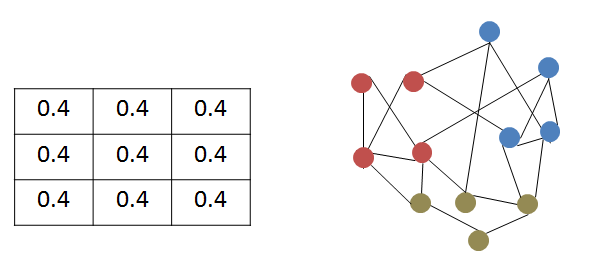
\includegraphics[width=1 \linewidth, height=5cm]{Erdos-Renyi.PNG} 
\caption{Example of SBM with equal probabilities}
\label{fig:erdos}
\end{figure}

\begin{figure}[ht]
\centering
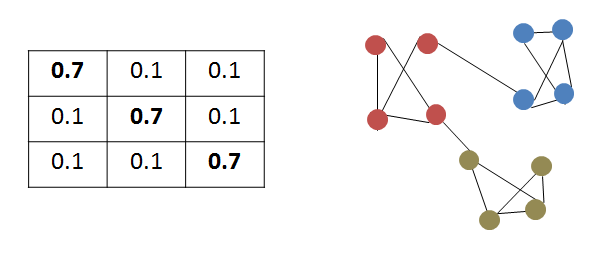
\includegraphics[width=1 \linewidth, height=5cm]{sbm.PNG} 
\caption{Example of SBM with assortative communities}
\label{fig:sbm}
\end{figure}

\subsection{Description of Experiments}

As mention in section \ref{chap:4}, the simulator was implemented in Elixir 1.6. The topology generator used to create network topology is an open source software written in Python under MIT license. Some modifications were done to the generator, for instance, compute the probability only for the upper triangular adjacency matrix of the topology, modified the parameters, customised the file format for store the topologies and some other minors modifications. 

The tests were run in a computer with processor Intel(R) Core(TM) i5--4210U of 1.7 and 2.4 GHz and RAM memory of 8 GB with additional 8 GB of SWAP. The operating system was a Linux 64 bit Debian base.


The value for $p$ was chosen to make sure that the generated graph is connected for the \textit{SBM}. Note that the algorithm for \textit{MIS} does not require this condition because it still finds the solution for a disconnected graph. However, the Beta Synchronizer construct a rooted spanning tree over the topology in order to send \textbf{safe} and \textbf{go} messages to the root and from it, so if the topology is not connected the rooted spanning tree can not be constructed. In order to maintain the same topologies for every simulation, the generated graphs are always connected.  

The steps to perform the experiments are enumerated below:

\begin{enumerate}
\item Implementation of the synchronizers Alpha and Beta.
\item Implementation of the Maximal Independent Set algorithm using the simulation developed in step 1.
\item Implementation of the Maximal Independent Set Algorithm using a global synchronization technique.
\item Create the topology with the Stochastic Block Model according to the description in the section \ref{sec:topology}.
\item Run N times the synchronous algorithm for the \textit{MIS} and saves the results for each synchronizer technique (Alpha, Beta and Global).
\item Compute the average and calculate the results.
\end{enumerate}




% \newpage

\section{Result Evaluation}
\label{chap:6}
Regarding the network topologies, ten different topologies were generated with the Stochastic Block Model for $n = 64, 256, 512,..., 32768$. The number of blocks $k$ was set to $\log n$. For the probability matrix the values used were $p = 7{\tfrac {\ln n}{n}}$ for the diagonal of the matrix and  $p\prime = {\tfrac {10}{n}}$ for values out of the diagonal . The values for the parameters are similar to the values used in \cite{kothapalli2013analysis}.

First, the result of the evaluation of the \textit{MIS} algorithm are presented. Then, the analysis of the synchronisation techniques and finally the conclusion of the evaluation.

% The results presented are the average of 10 executions of the simulation for each topology. For the \textit{MIS} algorithm it is important to measure the average of the execution because the algorithm is randomised and the unpredictable behaviour of the asynchronous message passing at the bottom. In consequence, for a given topology it is possible to obtain different results. The results observed in the simulation show that the number of rounds is similar in different execution however in can be some important differences in the number of messages. These results are presented in the next section.


\subsection{Evaluation of MIS algorithm}

The figure \ref{fig:rounds_execution} shows the average number of round that takes on each topology to finish the \textit{MIS} algorithm. As seen is section '\ref{cap:2}, the time complexity of the algorithm is $O(\log N)$ round in expectation. The plot is compare with a logarithmic plot showing the similarity among the shape of the curves.


\begin{figure}[ht]
\centering
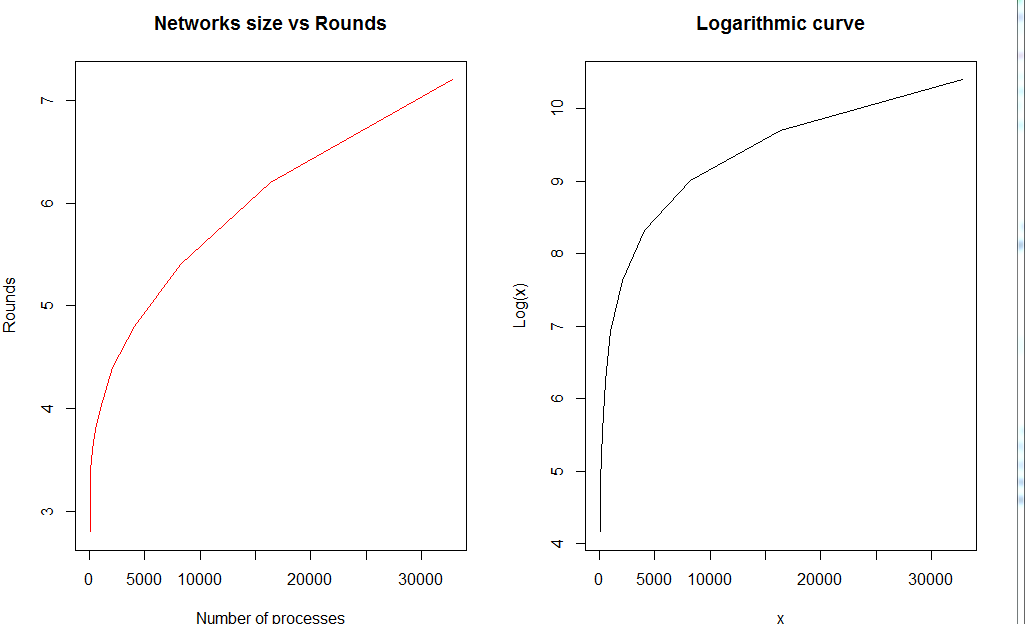
\includegraphics[width=1 \linewidth, height=5cm]{number_rounds.png} 
\caption{Rounds per execution}
\label{fig:rounds_execution}
\end{figure}

It is expected a progression in each round of the algorithm regarding the number of processes that finish the execution and become inactive. Once a processes finish the execution it output the final state (\textit{MIS} member or not). The progression of the algorithm can be seen in the figure \ref{fig:progression} for a network of 32768 processes. The blue line represents the number of processes that join the \textit{MIS}  per round and the red line shows the number of processes that are neighbours of some process that join the MIS. The figure \ref{fig:actives}, shows the total number of processes that are active in each round for the same topology. 

\begin{figure}[ht]
\centering
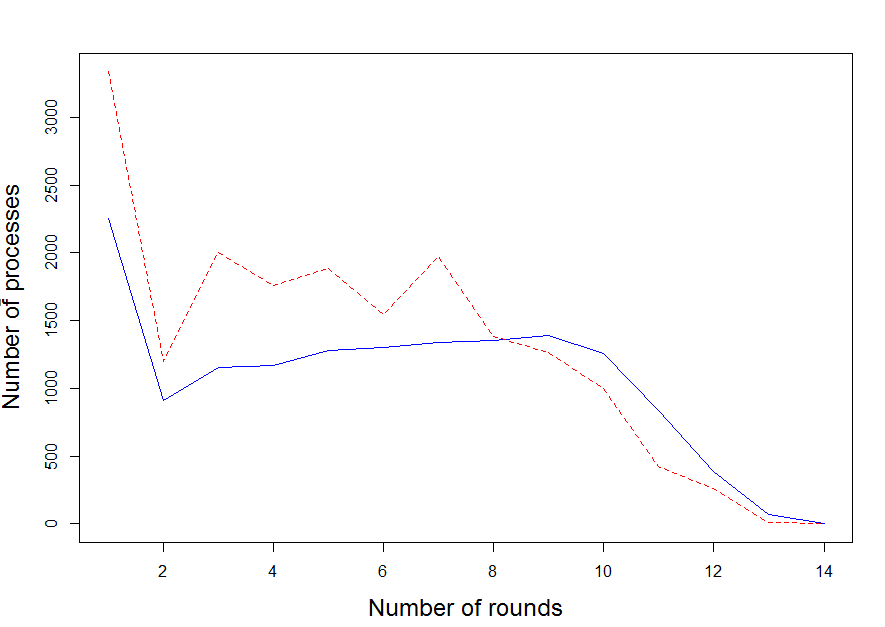
\includegraphics[width=0.7 \linewidth, height=5cm]{progress.PNG} 
\caption{Numbers of processes that finish the execution per round}
\label{fig:progression}
\end{figure}

\begin{figure}[ht]
\centering
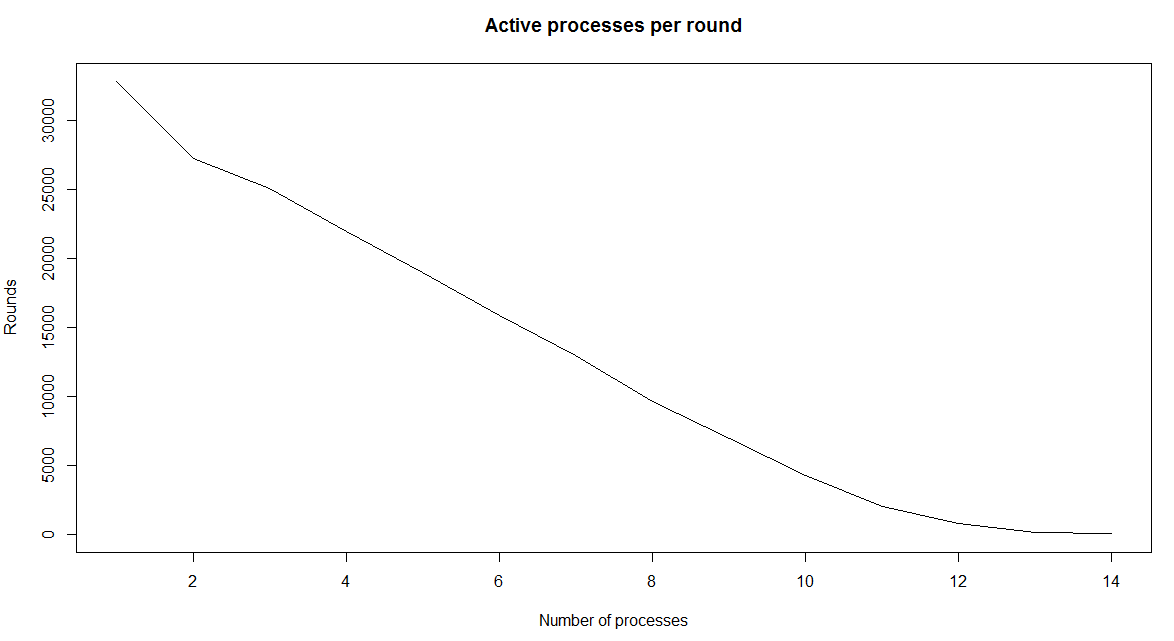
\includegraphics[width=0.7 \linewidth, height=5cm]{actives_round.PNG} 
\caption{Numbers of processes that finish the execution per round}
\label{fig:actives}
\end{figure}


\begin{figure}[ht]
\centering
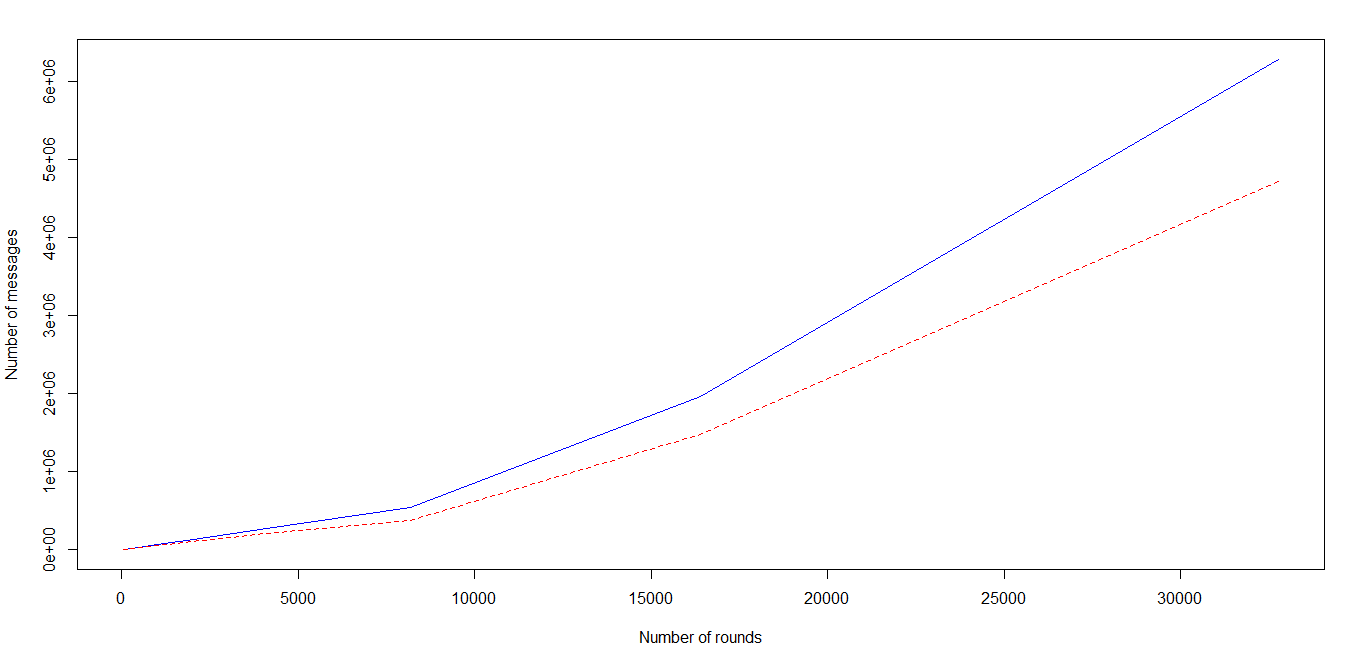
\includegraphics[width=0.7 \linewidth, height=5cm]{total_messages.PNG} 
\caption{Comparison between messages send for the protocol and the Global Synchronizer}
\label{fig:total_msg}
\end{figure}


 
\subsection{Evaluation of Synchronizers}

In this section ...

\subsection{Conclusions}

In this dissertation, the problem of finding the Maximal Independent Set in general graphs was studied. Distributed algorithms provide better time complexity than sequential algorithm. For distributed algorithm, it is assumed that the communication system is synchronous. In general, algorithms in synchronous system are easy to design and have lower complexity, therefore a distributed synchronous algorithm was implemented in order to analyse time and message complexity for the \textit{MIS} problem.


% \newpage

\section{Self Assessment}
\label{chap:7}
% \newpage


\bibliographystyle{plain}
\bibliography{bibliography}
\end{document}
